\documentclass[paper=a4, fontsize=11pt]{scrartcl}
\usepackage[T1]{fontenc}
\usepackage[utf8]{inputenc}
\usepackage{lmodern}
\usepackage{multirow}
\usepackage[table,xcdraw]{xcolor}
\usepackage[spanish]{babel}
\usepackage{cite}
\usepackage{amsmath,amsfonts,amsthm} % Math packages
\usepackage{graphics,graphicx, float} %para incluir imágenes y colocarlas
\usepackage[backref,colorlinks=true,linkcolor=black,urlcolor=blue,citecolor=blue]{hyperref} %Para crear enlaces en el pdf
\usepackage{url}
\usepackage[shortlabels]{enumitem}
\usepackage{appendix}
\usepackage{eurosym}
\usepackage{epsfig}
\usepackage{caption}
\usepackage{subcaption}

\usepackage{xcolor}
\usepackage{framed}
\definecolor{shadecolor}{RGB}{239, 251, 255}

\usepackage{listings}
\usepackage{color}

\definecolor{dkgreen}{rgb}{0,0.6,0}
\definecolor{gray}{rgb}{0.5,0.5,0.5}
\definecolor{mauve}{rgb}{0.58,0,0.82}
\definecolor{lgrey}{rgb}{0.9,0.9,0.9}


\lstset{frame=tb,
  language=C++,
  aboveskip=3mm,
  belowskip=3mm,
  showstringspaces=false,
  columns=flexible,
  basicstyle={\small\ttfamily},
  numbers=none,
  numberstyle=\tiny\color{gray},
  keywordstyle=\color{blue},
  commentstyle=\color{dkgreen},
  stringstyle=\color{mauve},
  breaklines=true,
  breakatwhitespace=true,
  tabsize=3
}

\renewcommand{\appendixname}{Anexo}
\renewcommand{\appendixtocname}{Anexo}
\renewcommand{\appendixpagename}{Anexo}

\numberwithin{figure}{section} % Number figures within sections (i.e. 1.1, 1.2, 2.1, 2.2 instead of 1, 2, 3, 4)
\numberwithin{table}{section} % Number tables within sections (i.e. 1.1, 1.2, 2.1, 2.2 instead of 1, 2, 3, 4)
\newcommand{\horrule}[1]{\rule{\linewidth}{#1}} % Create horizontal rule command with 1 argument of height

\title{
    \normalfont \normalsize
    \textsc{{\textbf{Algorítmica (2016-2017)}} \\ Grado en Ingeniería Informática \\ Universidad de Granada} \\ [25pt] % Your university, school and/or department name(s)
    \horrule{0.5pt} \\[0.4cm] % Thin top horizontal rule
    \huge Memoria Práctica 4: Backtracking y Branch & Bound\\ % The assignment title
    \horrule{2pt} \\[0.5cm] % Thick bottom horizontal rule
}
\author{Antonio de la Vega Jiménez }

%*************************************************************


\begin{document}

\maketitle % Muestra el Título
\newpage %inserta un salto de página
\tableofcontents % para generar el índice de contenidos
\listoffigures
\newpage

%*************************************************************

\section{Información PC usado}

\subsection{Hardware}
El hardware usado tiene las siguientes características:
\begin{itemize}
  \item \textbf{CPU:} \texttt{Intel(R) Core(TM) i5-4210U CPU}
  \item \textbf{Velocidad reloj:} \texttt{1.70 GHz}
  \item \textbf{Caché:} \texttt{3072 KB}
  \item \textbf{RAM:} \texttt{12190176 kB  }
\end{itemize}
\subsection{Software}
\subsubsection{Sistema operativo}
\begin{itemize}
  \item \textbf{SO:} \texttt{Manjaro Linux}
  \item \textbf{Kernel:}\texttt{ 4.9.24-1-MANJARO}
\end{itemize}
\subsubsection{Compilador}
\begin{itemize}
  \item \textbf{Versión compilador:} \texttt{g++ (GCC) 6.3.1 20170306}
\end{itemize}

\section{Suma hasta un número}

\subsection{Algoritmo voraz (Greedy)}

Este algoritmo no siempre encuentra la solución, por ejemplo si los candidatos son $ C = { 10 , 5 , 3 , 3 }  $ y queremos acumular $ M = 16 $,
este algoritmo cogerá el subconjunto $ S = { 10, 5} $ que no es la solución óptima.


El código usado es el mostrado a continuación

\begin{lstlisting}
vector<int> solucion_voraz(vector<int> candidatos, int obj) {
    vector<int> solucion;
    int acumulado = 0;

    sort(candidatos.begin(),candidatos.end());
    reverse(candidatos.begin(),candidatos.end());

    for(int i: candidatos) {       //selecion
        if(acumulado+i <= obj) {   //factible
            solucion.push_back(i); //aniadir
            acumulado+=i; 
        }

        if(acumulado == obj)
            break;
    }

    return solucion;
}
\end{lstlisting}

\subsubsection{Eficiencia teórica}

 Para obtener la eficiencia observamos que el algoritmo ordena el vector y luego simplemente lo recorre:
 
 La implementación de la funcion sort de la STL tiene una eficiencia:

  \begin{equation}
      O(n*log_2{n})
  \end{equation}

Y el resto del código de la función solucion\_voraz, tiene una eficiencia $ O(n) $ en el peor caso y $ O(1) $ en el mejor caso.

Por lo cual la eficiencia del algoritmo es:
 \begin{equation}
      O(n*log_2{n})
  \end{equation}

 
\subsubsection{Eficiencia empírica}

Al representar los datos obtenemos la siguiente gráfica:

\begin{figure}[H]
    \begin{center}
        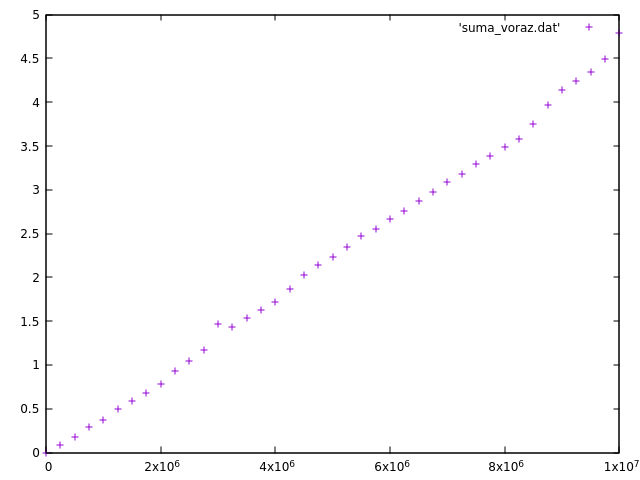
\includegraphics[scale=0.7]{imagenes/suma_voraz.png}
        \caption{Tiempos de ejecución.}
        \label{fig2}
    \end{center}
\end{figure}

\subsubsection{Ajuste curva teórica a empírica}

En este paso realizamos el siguiente ajuste:
\begin{shaded*}
\begin{verbatim}
gnuplot> f(x) = a*x*(log(x)/log(2))
gnuplot> fit f(x) 'suma_voraz.dat' via a

\end{verbatim}
\end{shaded*}

De forma que obtenemos los siguientes parámetros:

\begin{shaded*}
\begin{verbatim}
Final set of parameters            Asymptotic Standard Error
=======================            ==========================
a               = 1.90872e-08      +/- 5.685e-11    (0.2978%)
\end{verbatim}
\end{shaded*}

Y finalmente obtenemos la siguiente función ajustada:
\begin{figure}[H]
    \begin{center}
        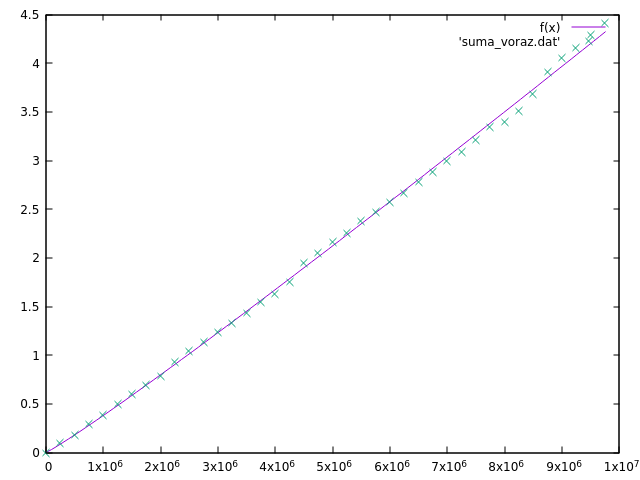
\includegraphics[scale=0.7]{imagenes/suma_voraz_adj.png}
        \caption{Ajuste eficiencia teórica y empírica.}
        \label{fig3}
    \end{center}
\end{figure}

%*************************************
%*************************************
%*************************************
%*************************************



\subsection{Algoritmo con programación dinámica}


Ecuación de recurrencia:

\begin{equation}
    K(k,m) =
\left\{
	\begin{array}{ll}
		0 & \mbox{if } m = 0 \\
		m & \mbox{if } k = 0 \\
		K(k-1,m) & \mbox{if } k > m \\
	    min( K(k-1,m), K(k-1,m-k)) & en otro caso
	\end{array}
\right.
\end{equation}



El código usado es el mostrado a continuación

\begin{lstlisting}
vector<int> rellenarTabla(vector<vector<int> > &tabla, vector<int> c, int obj) {

    for(int i = 0; i< tabla[0].size(); i++) {
        tabla[0][i] = i;
    }

    for(int i = 1; i < tabla.size(); i++) {
        for( int j = 0; j < tabla[i].size(); j++) {
            if(i == 0) {
                tabla[i][j] = 0;
            } else if (c[i] == 0) {
                tabla[i][j] = j;
            } else if (c[i] > j) {
                tabla[i][j] = tabla[i-1][j];
            } else {
                tabla[i][j] = min( tabla[i-1][j], tabla[i-1][j-c[i]]);
            }
        }
    }

    vector <int> solucion;

    int i,j;
    i = c.size()-1;
    j = obj;

    //recomponer la solución
    while(j != 0 && i != 0) {
        if(tabla[i-1][j] == tabla[i][j]) {
            i = i -1;
        } else {
            solucion.push_back(c[i]);
            j = j-c[i];
            i = i -1;
        }
    }

    return solucion;
}
\end{lstlisting}


\subsubsection{Eficiencia teórica}

La eficiencia depende del tamaño de la matriz, si tenemos n elementos y queremos obtener un valor m, la eficiencia es:

  \begin{equation}
      O(n*m)
  \end{equation}

\subsubsection{Eficiencia empírica}

Al representar los datos obtenemos la siguiente gráfica:

\begin{figure}[H]
    \begin{center}
        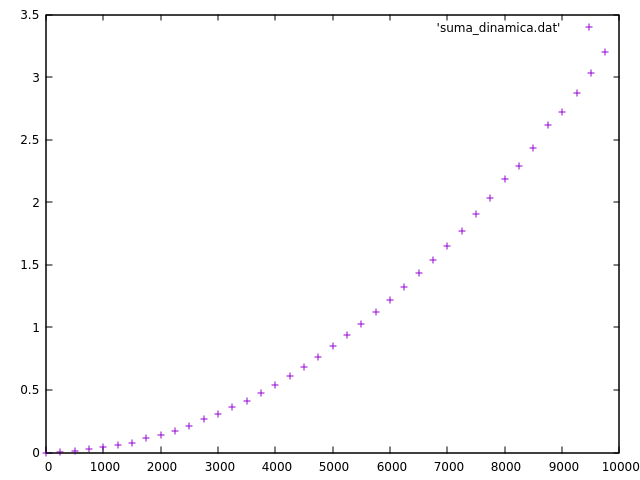
\includegraphics[scale=0.7]{imagenes/suma_dinamica.png}
        \caption{Tiempos de ejecución.}
        \label{fig19}
    \end{center}
\end{figure}

\subsubsection{Ajuste curva teórica a empírica}

\begin{shaded*}
\begin{verbatim}
gnuplot> f(x) = a*x*x + b*x + c
gnuplot> fit f(x) "suma_dinamica.dat" via a,b,c

\end{verbatim}
\end{shaded*}

De forma que obtenemos los siguientes parámetros:

\begin{shaded*}
\begin{verbatim}
Final set of parameters            Asymptotic Standard Error
=======================            ==========================
a               = 3.35471e-08      +/- 1.974e-10    (0.5884%)
b               = 1.48627e-06      +/- 1.991e-06    (134%)
c               = 0.00280063       +/- 0.004197     (149.9%)


\end{verbatim}
\end{shaded*}

Y finalmente obtenemos la siguiente función ajustada:
\begin{figure}[H]
    \begin{center}
        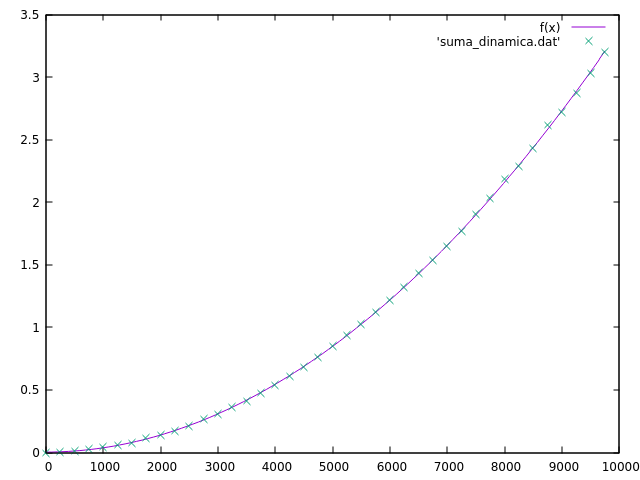
\includegraphics[scale=0.7]{imagenes/suma_dinamica_adj.png}
        \caption{Ajuste eficiencia teórica y empírica.}
        \label{fig20}
    \end{center}
\end{figure}


%*************************************
%*************************************
%*************************************
%*************************************

\section{Cifras}

\subsection{Algoritmo voraz (Greedy)}
El código usado es el mostrado a continuación

\begin{lstlisting}
void factible(vector<int> &sol, int candidato, int obj, int &acumulado) {

    int n = abs(obj - acumulado);
    int s = abs(obj - (candidato + acumulado));
    int r = abs(obj - (candidato - acumulado));
    int m = abs(obj - (candidato * acumulado));
    int d;
    if(candidato != 0 && acumulado != 0 && acumulado%candidato == 0) {
        d = abs(obj - int(acumulado/candidato));
    } else {
        d = numeric_limits<int>::max();
    }


    if(n <= s && n <= r && n <= m && n <= d ) {
        //nada
    } else if (s <= r && s <= m && s <= d) {
        sol.push_back(0);
        sol.push_back(candidato);
        acumulado+=candidato;

    } else if (r <= m && r <= d) {
        sol.push_back(1);
        sol.push_back(candidato);
        acumulado-=candidato;

    } else if (m <= d) {
        sol.push_back(2);
        sol.push_back(candidato);
        acumulado*=candidato;

    } else {
        sol.push_back(3);
        sol.push_back(candidato);
        acumulado/=candidato;
    }

    return;
}

vector<int> solucion_voraz(vector<int> &candidatos, int obj) {
    vector<int> solucion;
    int acumulado = 0;
    bool fin = false;

    for(int i = 0; i < candidatos.size() && !fin; i++) {
        factible(solucion,candidatos[i],obj,acumulado);

        if(acumulado == obj)
            fin = true;
    }
    return solucion;
}
\end{lstlisting}

\subsubsection{Eficiencia teórica}

 Para obtener la eficiencia observamos que el algoritmo recorre el vector y la función factible (que también se encarga de añadir a la solución) es constante, por lo tanto la eficiencia es:
 
  \begin{equation}
      O(n)
  \end{equation}

 
\subsubsection{Eficiencia empírica}

Al representar los datos obtenemos la siguiente gráfica:

\begin{figure}[H]
    \begin{center}
        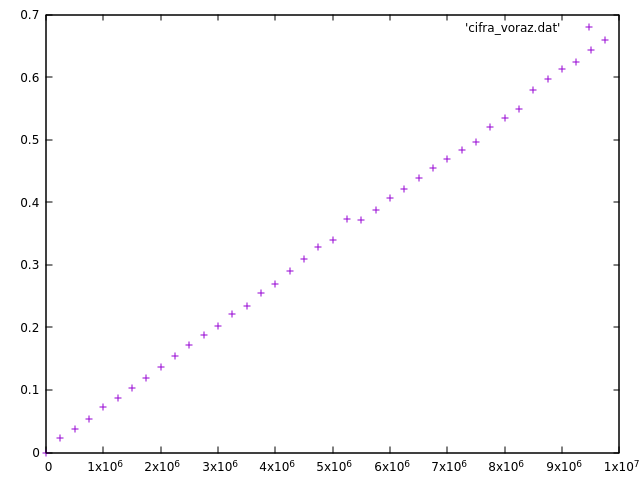
\includegraphics[scale=0.7]{imagenes/cifra_voraz.png}
        \caption{Tiempos de ejecución.}
        \label{fig2}
    \end{center}
\end{figure}

\subsubsection{Ajuste curva teórica a empírica}

En este paso realizamos el siguiente ajuste:
\begin{shaded*}
\begin{verbatim}
gnuplot> f(x) = a*x+b
gnuplot> fit f(x) 'cifra_voraz.dat' via a,b

\end{verbatim}
\end{shaded*}

De forma que obtenemos los siguientes parámetros:

\begin{shaded*}
\begin{verbatim}
Final set of parameters            Asymptotic Standard Error
=======================            ==========================
a               = 6.76338e-08      +/- 2.744e-10    (0.4058%)
b               = 1.53036e-06      +/- 0.001555     (1.016e+05%)

\end{verbatim}
\end{shaded*}

Y finalmente obtenemos la siguiente función ajustada:
\begin{figure}[H]
    \begin{center}
        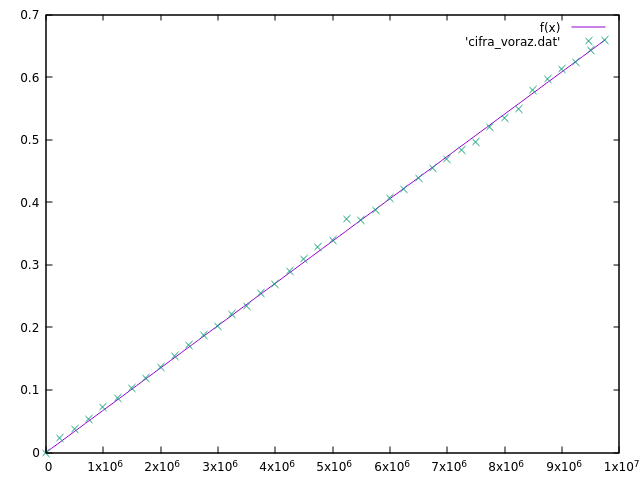
\includegraphics[scale=0.7]{imagenes/cifra_voraz_adj.png}
        \caption{Ajuste eficiencia teórica y empírica.}
        \label{fig3}
    \end{center}
\end{figure}

%*************************************
%*************************************
%*************************************
%*************************************

\subsection{Algoritmo con programación dinámica}


Ecuación de recurrencia:

\begin{equation}
    K(k,m) =
\left\{
	\begin{array}{ll}
		0 & \mbox{if } m = 0 \\
		m & \mbox{if } k = 0 \\
		\inf & \mbox{if } fuera limites\\
	    min( K(k-1,m), K(k-1,m-k), \\K(k-1,m+k), K(k-1,m*k),\\ K(k-1,m/k)) & en otro caso
	\end{array}
\right.
\end{equation}



El código usado es el mostrado a continuación

\begin{lstlisting}
vector<pair<char,int> > rellenarTabla(vector<vector<pair<char,int> > > &tabla, vector<int> c, int obj) {

    int limit = std::numeric_limits<int>::max();
    pair<char,int> nada,suma,resta,multiplicacion,division,MIN;

    for(unsigned int i = 0; i< tabla[0].size(); i++) {
        tabla[0][i].second = i;
        tabla[0][i].first = '.';
    }

    for(int i = 1; i < tabla.size(); i++) {
        for( int j = 0; j < tabla[i].size(); j++) {
            if(i == 0) {
                tabla[i][j].second = 0;
                tabla[i][j].first = '.';
            } else if (c[i] == 0) {
                tabla[i][j].second = j;
                tabla[i][j].first = '.';

            } else {

                nada.second = tabla[i-1][j].second;
                nada.first = '.';

                if(j-c[i] < 0) {
                    suma.second = limit;
                    suma.first = '+';
                } else {
                    suma.second = tabla[i-1][j-c[i]].second;
                    suma.first = '+';
                }

                if(j+c[i] >= tabla[0].size()-1) {
                    resta.second = limit;
                    resta.first = '-';
                } else {
                    resta.second = tabla[i-1][j+c[i]].second;
                    resta.first = '-';
                }

                if(j*c[i] >= tabla[0].size()-1) {
                    division.second = limit;
                    division.first = '/';
                } else {
                    division.second = tabla[i-1][j*c[i]].second;
                    division.first = '/';
                }

                if(j%c[i] != 0) {
                    multiplicacion.second = limit;
                    multiplicacion.first = '*';
                } else {
                    multiplicacion.second = tabla[i-1][j/c[i]].second;
                    multiplicacion.first = '*';
                }

                MIN = minimo(nada,suma,resta,division,multiplicacion);

                tabla[i][j] = MIN;
            }
        }
    }

    vector <pair<char,int> > solucion;

    //recomponer la solución
    int i,j;
    i = c.size()-1;
    j = obj;


    while(j != 0 && i != 0) {
        if(tabla[i-1][j].second == tabla[i][j].second) {
            i = i -1;
        } else {
            solucion.push_back(make_pair(tabla[i][j].first, c[i]));
            j = j-c[i];
            i = i -1;
        }
    }


    return solucion;
}

\end{lstlisting}


\subsubsection{Eficiencia teórica}

La eficiencia depende del tamaño de la matriz, si tenemos n elementos y queremos obtener un valor m, la eficiencia es:

  \begin{equation}
      O(max(n)*m)
  \end{equation}

\subsubsection{Eficiencia empírica}

Al representar los datos obtenemos la siguiente gráfica:

\begin{figure}[H]
    \begin{center}
        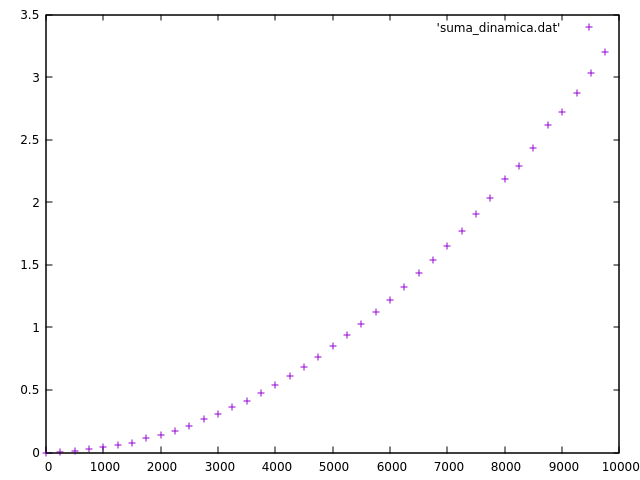
\includegraphics[scale=0.7]{imagenes/suma_dinamica.png}
        \caption{Tiempos de ejecución.}
        \label{fig19}
    \end{center}
\end{figure}

\subsubsection{Ajuste curva teórica a empírica}

\begin{shaded*}
\begin{verbatim}
gnuplot> f(x) = a*x*x + b*x + c
gnuplot> fit f(x) "suma_dinamica.dat" via a,b,c

\end{verbatim}
\end{shaded*}

De forma que obtenemos los siguientes parámetros:

\begin{shaded*}
\begin{verbatim}
Final set of parameters            Asymptotic Standard Error
=======================            ==========================
a               = 3.35471e-08      +/- 1.974e-10    (0.5884%)
b               = 1.48627e-06      +/- 1.991e-06    (134%)
c               = 0.00280063       +/- 0.004197     (149.9%)


\end{verbatim}
\end{shaded*}

Y finalmente obtenemos la siguiente función ajustada:
\begin{figure}[H]
    \begin{center}
        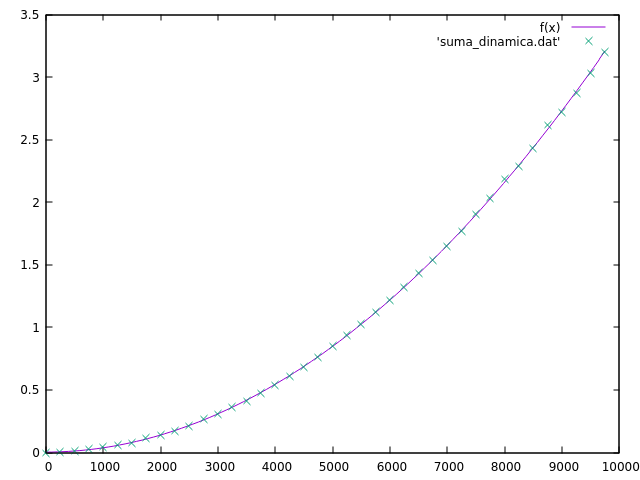
\includegraphics[scale=0.7]{imagenes/suma_dinamica_adj.png}
        \caption{Ajuste eficiencia teórica y empírica.}
        \label{fig20}
    \end{center}
\end{figure}


%*************************************************************
\newpage

\end{document}
